%=======================================================================
% Declarações iniciais identificando a classe de documento e
% selecionando alguns pacotes adicionais.
%
% As opções disponíveis (separe-as com vírgulas, sem espaço) são:
% - twoside: Formata o documento para impressão frente-e-verso
%   (o default é somente-frente)
% - english,brazilian,french,german,etc.: idiomas usados no documento.
%   Deve ser colocado por último o idioma principal.
%=======================================================================
\documentclass[twoside,english,brazilian]{UNISINOSmonografia}
\usepackage[utf8]{inputenc} % charset do texto (utf8, latin1, etc.)
\usepackage[T1]{fontenc} % encoding da fonte (afeta a sep. de sílabas)
\usepackage{graphicx} % comandos para gráficos e inclusão de figuras
\usepackage{bibentry} % para inserir refs. bib. no meio do texto

\graphicspath{ {./images/} }

%=======================================================================
% Escolha do sistema para geração de referências bibliográficas.
%
% O default é usar o estilo unisinos.bst.  Comente a definição abaixo
% e descomente a linha seguinte para usar o estilo do ABNTeX (é
% necessário ter esse pacote instalado).
%
% A vantagem do unisinos.bst é que ele permite o uso de um arquivo .bib
% seguindo as orientações tradicionais do BibTeX (veja essas orientações
% em http://ctan.tug.org/tex-archive/biblio/bibtex/contrib/doc/btxdoc.pdf).
% Entretanto, o estilo não suporta algumas citações mais exóticas como
% apud.  Para isso, use o ABNTeX, mas esteja ciente de que muitas de
% suas referências serão incompatíveis com os estilos tradicionais do
% BibTeX como plain, alpha, ieeetr, entre outros.
%=======================================================================
\unisinosbst
%\usepackage[alf]{abntcite}


%=======================================================================
% Dados gerais sobre o trabalho.
%=======================================================================
\autor{Aubin}{Mateus Rauback}
\author{Mateus Rauback Aubin}
\titulo{
Um Sistema de Gestão de Dispositivos Inteligentes 
Baseado em Protocolos de Gerência de Redes Voltado Para a 
Internet das Coisas
}
%\subtitulo{Versão \LaTeX}
\orientador[Prof.~Dr.]{Ávila}{Rafael Bohrer}
%\coorientador[Prof.~Dr.]{Lamport}{Leslie}
\local{São Leopoldo}
\ano{2013}

%% dados específicos para monografia de Graduação
\unidade{Unidade Acadêmica Graduação}
\curso{Curso de Bacharelado em Ciência da Computação}
\natureza{
Trabalho de Conclusão de Curso apresentado como requisito parcial
para a obtenção do título de Bacharel em Ciência da Computação
pela Universidade do Vale do Rio dos Sinos --- UNISINOS
}


%=======================================================================
% Palavras Chave.
%
% Deve ser fornecida para cada idioma.
%=======================================================================
\palavrachave{brazilian}{Internet das Coisas}
\palavrachave{english}{Internet of Things}

\palavrachave{brazilian}{Gerência de Redes}
\palavrachave{english}{Network Management}

\palavrachave{brazilian}{Protocolos de Rede}
\palavrachave{english}{Network Protocols}


%=======================================================================
% Início do documento.
%=======================================================================
\begin{document}
\capa
\folhaderosto


%=======================================================================
% Dedicatória (opcional).
%
% O texto é normalmente colocado na parte de baixo da página, alinhado
% à direita.  Mas a formatação é basicamente livre.  Só não se escreve
% a palavra 'dedicatória'.
%=======================================================================
%\begin{dedicatoria}
%Aos nossos pais.\\[4ex] % quebra a linha dando um espaçamento maior
%\begin{itshape} % faz o texto ficar em itálico
%If I have seen farther than others,\\
%it is because I stood on the shoulders of giants.\\
%\end{itshape}
%--- \textsc{Sir Isaac Newton} % \textsc é o "small caps"
%\end{dedicatoria}


%=======================================================================
% Agradecimentos (opcional).
%=======================================================================
%\begin{agradecimentos}
%Obrigado!
%\end{agradecimentos}


%=======================================================================
% Epígrafe (opcional).
%
% ``[...] o autor apresenta uma citação, seguida de indicação de autoria,
% relacionada com a matéria tratada no corpo do trabalho. Podem, também,
% constar epígrafes nas folhas de aberturas das seções primárias.''
%=======================================================================
%\begin{epigrafe}
%``\textit{Ninguém abre um livro sem que aprenda alguma coisa}''.\\
%(Anônimo)
%\end{epigrafe}


%=======================================================================
% Resumo em Português.
%
% A recomendação é para 150 a 500 palavras.
%=======================================================================
%\begin{abstract}
%Aqui vai o resumo
%\end{abstract}


%=======================================================================
% Resumo em língua estrangeira (obrigatório somente para teses e
% dissertações).
%
% O idioma usado aqui deve necessariamente aparecer nos parâmetros do
% \documentclass, no início do documento.
%=======================================================================
%\begin{otherlanguage}{english}
%\begin{abstract}
%Abstract goes here
%\end{abstract}
%\end{otherlanguage}


%=======================================================================
% Lista de Figuras (opcional).
%=======================================================================
%\listoffigures


%=======================================================================
% Lista de Tabelas (opcional).
%=======================================================================
%\listoftables


%=======================================================================
% Lista de Abreviaturas (opcional).
%
% Deve ser passada como parâmetro a maior das abreviaturas utilizadas.
%=======================================================================
%\begin{listadeabreviaturas}{seg., segs.}
%\item[ampl.] ampliado, -a
%\item[atual.] atualizado, -a
%\item[coord.] coordenador
%\item[N.~T.] Novo Testamento
%\item[seg., segs.] seguinte, -s
%\end{listadeabreviaturas}


%=======================================================================
% Lista de Siglas (opcional).
%
% Deve ser passada como parâmetro a maior das siglas utilizadas.
%=======================================================================
\begin{listadesiglas}{IoT}
\item[IoT] Internet of Things
%\item[CAPES] Coordenação de Aperfeiçoamento de Pessoal de Nível Superior
%\item[FAPERGS] Fundação de Amparo à Pesquisa do Estado do Rio Grande do Sul
\end{listadesiglas}


%=======================================================================
% Lista de Símbolos (opcional).
%
% Deve ser passado o maior (mais largo) dos símbolos utilizados.
%=======================================================================
%\begin{listadesimbolos}{Ca}
%\item[\textsuperscript{o}C] Graus Celsius
%\item[Al] Alumínio
%\item[Ca] Cálcio
%\end{listadesimbolos}


%=======================================================================
% Sumário
%=======================================================================
\tableofcontents


%=======================================================================
% Introdução
%=======================================================================
\chapter{1 Introdução}

% as epígrafes nos capítulos são opcionais
\epigrafecap{in the nineteenth century, machines learned to do; in the twentieth century, they learned to think; and in the twenty-first century, they are learning to perceive -- they actually sense and respond.}
{\citetexto{Sundmaeker2010}}

	O contínuo aumento na capacidade de processamento dos dispositivos 
	computacionais aliado a redução de custos possibilitou uma nova revolução 
	tecnológica. Munidos de circuitos integrados e microchips, cada vez mais 
	os computadores avançam em direção à ubiquidade. 
	
	No atual cenário tecnológico já é possível colocar em prática, de maneira 
	economicamente viável, algumas das ideias vislumbradas por 
	\citetexto{Weiser1991}. A integração entre dispositivos computacionais e a 
	vida cotidiana apresenta um grande desafio para diversas áreas do 
	conhecimento, entretanto, as barreiras estão gradualmente diminuindo,
	possibilitando a criação de novos produtos e soluções para os mais 
	diversos problemas. 
	
	Apesar de não ser uma ideia nova, a implementação de uma Internet das 
	Coisas não era viável devido a fatores como a complexidade e o custo da 
	criação de uma rede de dispositivos embarcados em objetos do dia-a-dia. 
	Tomando por referência a lei de \citetexto{Moore1965}, que dita que o 
	número de transistores em um circuito integrado dobra aproximadamente a 
	cada dezoito meses, é improvável que esta tendência, de dispositivos cada 
	vez menores e mais baratos, se reverta.
	
	Diversas são as semelhanças entre a Internet das Coisas e Redes de 
	Sensores sem Fio (WSN), porém, enquanto as WSNs \cite{Sakthidharan2012} 
	são implantadas principalmente com o intuito de monitorar eventos em um 
	ambiente, a Internet das Coisas expande este conceito ao próximo nível. Ao 
	possibilitar que cada dispositivo seja individualmente endereçável na 
	Internet, o compartilhamento de informações entre sistemas é favorecido, 
	resultando em uma modalidade de comunicação chamada por 
	\citetexto{ETSI2010} de comunicação Máquina-a-Máquina (M2M).

	\section{Internet das Coisas}
	
\subsection{Origem}

%TODO RFID
%TODO WSN
%TODO Gateways para conectar a Internet \cite{Zhu2010}
%TODO IPv6 e a possibilidade de endereçar todo objeto \cite{Sundmaeker2010}p15
%TODO Smart Objects
	
\subsection{Definição}
	
		Diversas são as definições disponíveis para o termo Internet das 
		Coisas (IoT), \citetexto{Atzori2010b} atribuem a grande variedade de 
		definições às diferentes visões que cada organização, dependendo dos 
		seus objetivos, tem, geralmente sendo orientadas a Internet ou as 
		coisas. Apesar das diferenças o conceito de IoT é, para 
		\citetexto{Coetzee2011}:
		
		\begin{quote}
			uma visão onde objetos se tornam parte da Internet: onde cada 
			objeto é unicamente identificável e acessível à rede, sua posição 
			e status conhecidos, onde serviços e inteligência são acrescidos a 
			esta Internet expandida, fundindo o mundo físico e o digital~
			\cite{Coetzee2011}.
		\end{quote}
		
		Segundo \citetexto{Sundmaeker2010}, dentre as mais citadas estão as 
		definições por Kevin \citetexto{Ashton2009} e David 
		\citetexto{Brock2001} do Auto-ID Labs e da União Internacional de 
		Telecomunicações, \citetexto{ITU2005}. Enquanto a primeira é focada na 
		identificação e detecção de objetos através do uso de RFIDs, a segunda 
		aborda uma definição mais ampla, detalhada a seguir.
		
		Em sua definição, a \citetexto{ITU2005} sugere que a Internet das 
		Coisas, através de suas tecnologias será capaz de conectar objetos de 
		maneira inteligente e sensorial, combinando avanços nos campos de:
		\begin{itemize}
			\item Identificação --- \textit{Tagging things}: Tecnologias para 
			reconhecimento e rastreamento de objetos, baseadas principalmente 
			em RFID. Possibilitam uma forma primitiva de integração entre o 
			real e o virtual.
			
			\item Sensores --- \textit{Feeling things}: Tecnologias 
			relacionadas a WSNs, utilizando-se dos conhecimentos já adquiridos 
			pelas pesquisas nesta área. Sensores ampliam a quantidade de 
			informações contextuais para aplicações, possibilitando um melhor 
			mapeamento do seu ambiente por meio de parâmetros como: 
			temperatura, luminosidade, vibração, nível de ruído e etc\ldots
			
			\item Sistemas embarcados --- \textit{Thinking things}: Refere-se 
			a crescente capacidade de embutir microcontroladores e 	
			processadores em objetos da vida cotidiana, efetivamente 
			possibilitando a criação de objetos inteligentes. Com a redução de 
			custo e tamanho, a substituição de circuitos de propósito 
			específico por processadores multipropósito é favorecida, criando 
			uma nova geração de objetos.
			
			\item Nanotecnologia --- \textit{Shrinking things}: Abordando o 
			impacto e as possibilidades do uso altamente difundido de 
			tecnologias de nano escala. Dentre as previsões estão circuitos 
			menores, mais econômicos e baratos, além do uso de novos 
			materiais, como grafeno e nanotubos, na fabricação destes 
			dispositivos.
		\end{itemize}
		
		Entretanto, a riqueza de possibilidades abertas pela IoT pode ser 
		explicada simplesmente pela análise individual de seus termos 
		constituintes, ou seja, a combinação de Internet e coisas. Segundo 
		\citetexto{Simpson2005}, no Oxford English Dictionary, a Internet é 
		``uma rede global de computadores provendo diversos serviços de 
		informação e comunicação, constituída de redes interconectadas usando 
		protocolos padronizados de comunicação''.
		
		Coisas, por outro lado, não tem uma definição precisa, podendo variar 
		conforme o contexto e o foco da aplicação. \citetexto{Coetzee2011} 
		apresentam uma definição abrangente direcionada para IoT:
		
		\begin{quote}
			A definição de ``coisas'' na visão da IoT é muito ampla e inclui 
			uma variedade de elementos físicos. Estes incluem objetos pessoais 
			que carregamos como \textit{smart phones}, \textit{tablets} e 
			câmeras digitais. Ela também inclui elementos em nosso ambiente 
			(seja em casa, no carro ou no trabalho) assim como coisas 
			equipadas com \textit{tags} (RFID ou outras) que se tornam 
			conectadas através de um portal de acesso (um \textit{smart 
			phone}, por exemplo).~
			\cite{Coetzee2011}.
		\end{quote}
		
		Identifica-se uma mudança gradual na definição do conceito de Internet 
		das Coisas, inicialmente contemplando apenas mecanismos de 
		identificação e, impulsionado pela evolução tecnológica, passando a 
		versar sobre dispositivos inteligentes e diretamente conectados à 
		Internet necessidade de intermediários. Segundo 
		\citetexto{Buckley2006} a transformação no conceito de IoT é resultado 
		tanto de avanços tecnológicos quanto de interesse mercadológico 
		impulsionado pelos potenciais benefícios.
		
% Based on the above view of “things” an enormous number of devices and things 
% will be connected to the Internet, each providing data and information and 
% some, even services.

\subsection{Importância}

		Uma vez estabelecida a definição de Internet das Coisas, é possível 
		compreender o impacto social e tecnológico deste conceito. A Internet 
		causou uma revolução na maneira com que compartilhamos informação e 
		conhecimento, gerando, de acordo com \citetexto{Carr2010}, mudanças 
		até mesmo em nossa estrutura cerebral.
		
		Classificada como a terceira onda da computação \cite{Register2013}, 
		os conceitos de IoT poderão ser aplicados a diversos setores 
		produtivos, desde a indústria ao setor público. Os possíveis 
		benefícios obtidos através de uma vasta rede de dispositivos 
		interconectados fez com que especialistas como \citetexto{Hung2012}, 
		da Gartner, classificassem IoT como um paradigma transformacional.
		
		\citetexto{Cisco2011} ressalta que a importância da IoT está 
		profundamente interligada na maneira como a humanidade se desenvolveu: 
		``Humanos evoluem porque se comunicam. Assim que o fogo foi descoberto 
		e compartilhado, por exemplo, ele não precisou ser redescoberto, 
		apenas comunicado''. Ainda sob este ponto de vista afirma que, com a 
		aplicação dos conceitos de IoT, haverá um aumento exponencial na 
		quantidade de dados disponível:
		
		\begin{quote}
			considere que a IoT representa a próxima evolução da Internet, 
			levando a um enorme salto na sua habilidade de coletar, analisar e 
			distribuir dados que podemos transformar em informação, 
			conhecimento e, finalmente, sabedoria.~
			\cite[p.~2]{Cisco2011}.
		\end{quote}
		
		%TODO Melhorar a figura
		\begin{figure}
			\caption{Hierarquia do conhecimento}
			\label{fig:wkid}
			\centering
			\begin{minipage}{.8\textwidth}
				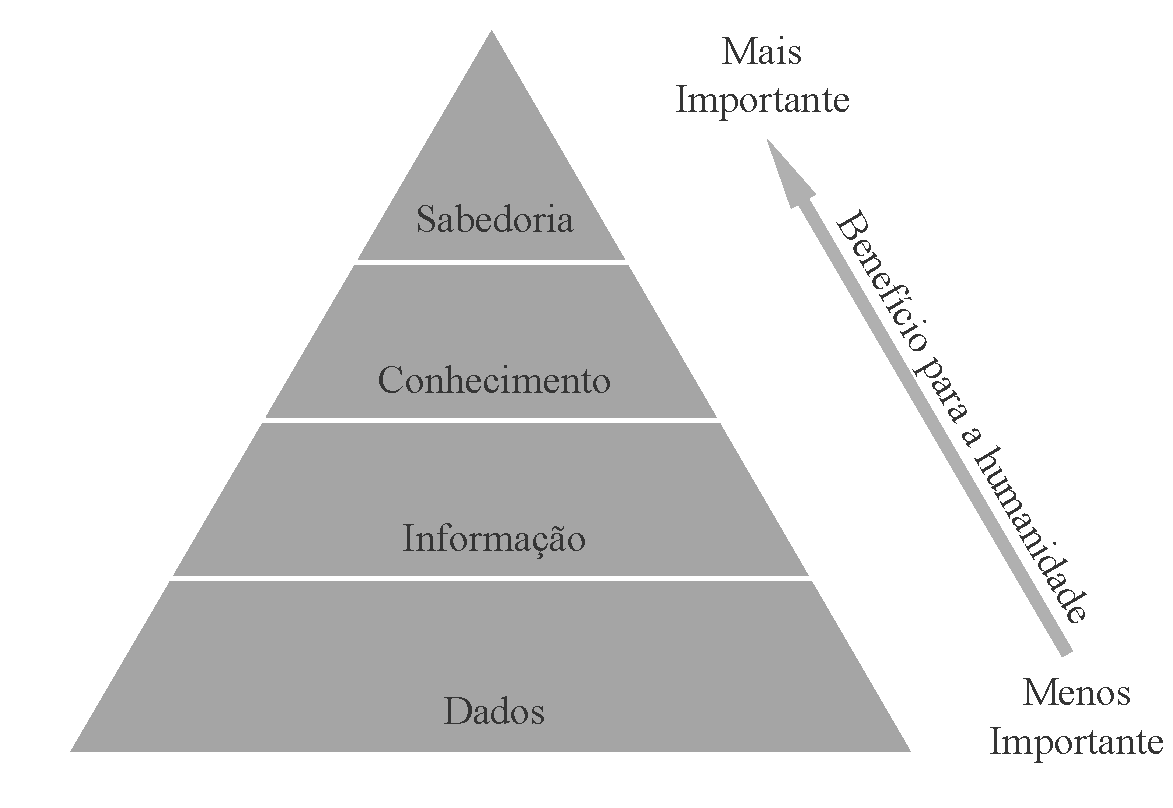
\includegraphics[width=\textwidth]{wkid}
				\fonte{\citetexto{Cisco2011}}
			\end{minipage}
		\end{figure}
		
		%TODO Medir & Otimizar (gestão de processos)
decisoes em tempo real a partir de leituras de sensores
alta resolução dos dados, possibilitando controle individual de recursos (big 
data)

		%TODO Relacionar com Big Data
		
		\citetexto{Cisco2011} estima que em 2015 haverão 25 bilhões de 
		dispositivos conectados a Internet e que apenas 5 anos depois, em 
		2020, este número chegará a casa de 50 bilhões.
		
\subsection{Desafios}

%TODO Tecnológicos: bateria, processamento, antenas, protocolos
%TODO Sociais: ética, privacidade (big brother)

\subsection{Oportunidades}

IBM Smarter Planet
HP?

inteligencia por agregação de dados
processos autonomos

explicar as principais vantagens do uso de IoT nos seguintes contextos
Industria
Meio Ambiente
Sociedade (governamental)
depois identificar e exemplificar os Application Domains \cite{Sundmaeker2010}


\section{Gerência de Redes}

	Impulsionada pelo crescimento e evolução das redes de computadores, as 
	técnicas de gerência de redes se tornaram fundamentais para garantir o 
	funcionamento e a qualidade dos serviços prestados. Cada vez mais 
	importantes para as atividades humanas, as redes de computadores, em 
	especial a Internet, ``têm catalizado a inovação e favorecido a emergência 
	de novos e disruptivos modelos de negócio'' \cite{Ding2009}.
	
	De acordo com \citetexto{Clemm2006}, a gerência de redes pode ser definida 
	como ``as atividades, métodos, procedimentos, e ferramentas que dizem 
	respeito a operação, administração, manutenção e provisionamento de 
	sistemas de rede''. Uma definição extensiva do conceito de gerência de 
	redes é fornecida por \citetexto{Ding2009}:
	
	\begin{quotation}
		a execução de um conjunto de funções requeridas para controlar, 
		planejar, alocar, implantar, coordenar, e monitorar os recursos de uma 
		rede de telecomunicações ou de computadores, incluindo a realização de 
		funções como planejamento inicial da rede, atribuição de frequências, 
		roteamento predefinido de tráfico para suportar balanceamento de 
		carga, autorização de distribuição de chaves criptográficas, gerência 
		de configuração, gerenciamento de falhas, gestão da segurança, 
		gerência de performance e gestão de contabilização.~
		\cite[p.~64]{Ding2009}.
	% defined as the execution of the set of functions required for 
	% controlling, planning, allocating, deploying, coordinating, and 
	% monitoring the resources of a telecommunications network or a computer 
	% network, including performing functions such as initial network 
	% planning, frequency allocation, predetermined traffic routing to 
	% support load balancing, cryptographic key distribution authorization, 
	% configuration management, fault management, security management, 
	% performance management, and accounting management.
	\end{quotation}

	O reconhecimento da importância das técnicas de gerência de redes provocou 
	esforços por parte de órgãos reguladores, como a Organização Internacional 
	para Padronização (ISO). Em sua normativa 7498-4, a \citetexto{ISO1989} 
	define as cinco principais categorias da gerência de redes, conhecido como 
	o modelo FCAPS:
	
	\begin{itemize}
		\item gerenciamento de falhas
		\item gerência de configuração
		\item gestão de contabilização
		\item gerência de performance
		\item gestão da segurança
	\end{itemize}
	
	Para que ocorra o gerenciamento de rede, são necessários, segundo 
	\cite{Ding2009}, três componentes principais:
	
	\begin{itemize}
		\item Centro de gerenciamento
		\item Dispositivo gerenciado
		\item Protocolo de gerenciamento
	\end{itemize}

\section{O Problema}

	Expor o problema da gestão dos objetos inteligentes e como a grande 
	quantidade
	de dispositivos vai deixar este problema ainda pior.
		
	Descrever os objetivos brevemente de maneira textual e depois colocá-los em
	forma de topicos\ldots


	\subsection{Objetivo Geral}
	
		Definir, projetar e desenvolver um sistema de gerencia de dispositivos 
		inteligentes utilizando-se de modelos e protocolos da gerência de 
		redes tradicional aplicado a Internet das Coisas.
	
	
	\subsection{Objetivos Específicos}
	
		\begin{itemize}
			\item 
				Aprofundar os conhecimentos sobre protocolos de Gerência de 
				Redes e sobre protocolos utilizados por dispositivos aplicados 
				à Internet das Coisas;
				
			\item
				Definir e projetar um conjunto de extensões voltadas à gestão 
				de dispositivos inteligentes de forma a melhor adaptar o 
				protocolo escolhido à proposta;
				
			\item
				Definir e projetar um software de Gerência de Redes com 
				suporte as extensões propostas.
				
		\end{itemize}


\chapter{2 Metodologia}
% FICA MAIS PARA O FINAL PARA DESCREVER OS PROXIMOS PASSOS NO DESENVOLVIMENTO
% DO TRABALHO...

	Um estudo abrangendo os principais protocolos de gerencia de redes e de 
	comunicação entre dispositivos inteligentes será realizado como ponto de 
	partida para o trabalho proposto. Este estudo tem por objetivo fazer um 
	levantamento dos protocolos de maior destaque em seu ramo, possibilitando 
	a criação de um panorama contendo as principais tecnologias.
	
	De posse destes dados será feita uma avaliação para decidir quais 
	protocolos apresentam as melhores características para atingir os 
	objetivos deste trabalho. Esta etapa visa selecionar quais tecnologias 
	serão utilizadas no restante do desenvolvimento do trabalho, de forma a 
	obter a maior contribuição científica possível.
	
	Nesta etapa ocorrerá uma análise das funcionalidades do protocolo de 
	gerencia de redes escolhido visando encontrar quais delas são úteis para o 
	paradigma de Internet das Coisas e, adicionalmente, serão sugeridas 
	melhorias específicas para este domínio de aplicação.
	
	Uma vez definido o conjunto de extensões necessárias ao protocolo de 
	gerencia de redes selecionado, será projetado um software capaz de 
	utilizar-se destas melhorias. Nesta etapa será criada a arquitetura do 
	sistema de gerencia de redes específico para a gestão de dispositivos 
	inteligentes.
	
	Finalmente serão efetivamente desenvolvidas as melhorias propostas. Nesta 
	etapa serão implementadas as melhorias ao protocolo de gerencia de redes e 
	será também desenvolvido o sistema de gerencia de redes aplicado a gestão 
	de dispositivos inteligentes no contexto de Internet das Coisas.


\chapter{3 Protocolos de Gerência de Redes}
% ABORDAR A LITERATURA CLASSICA EM UM MOMENTO, EXPLICANDO OS PRINCIPAIS CARAS 
% E AS DEFINIÇÕES.

% DEPOIS ABORDAR A PARTE DE ARTIGOS COM TRABALHOS RELACIONADOS O QUE FIZERAM
% RELACIONANDO IoT COM GERENCIA DE REDES

	Contextualizar o leitor com a utilidade e os objetivos de um protocolo
	de gerência de redes. Porque foram feitos, quais problemas resolvem,
	onde funcionam bem e onde não são tão bons (segurança, por exemplo).
	FCAPS\ldots
	
	Apresentar os protocolos principais, seus pontos fortes e fracos.
	
	
	
	\section{Modelo OSI (CMIP / CMOT)}

		Apresentar este protocolo
		
		
		
	\section{SNMP}

		Principal objeto de estudo do trabalho até o momento.
		Provavelmente será o protocolo escolhido.
		
		
	
	\section{WSDM}
	
	
	\section{Management By Delegation}
	
	
	\section{AgentX}
	
	
	\section{Outros?!}
	
	
	\section{Conclusão}
	
		Apresentar o melhor candidato pra receber as melhorias e justificar
		a escolha\ldots



\chapter{4 Proposta para IoT}

	Abordar neste capítulo as necessidades específicas de IoT e suas 
	características.
	
	Apresentar as dificuldades (problemas) que levarão para as propostas
	de como resolvê-las com as extensões ao protocolo.
	
	
	\section{Multicast}
		
		Propor o uso de multicast para enviar diversos comandos aos objetos
		disponíveis na rede.
		
		
	\section{Tageamento de Objetos}
		
		Propor um sistema para tagear objetos com base em características
		arbitrárias definidas pelo fabricante e pelo usuário.
		
		Quero enviar este comando para todos os objetos elétricos, para
		todos que estão na cozinha, para todos os sensores...
		
		
	\section{Compressão de Headers}
		
		Conforme feito por \cite{Choi2009}
		
		
	\section{Compressão de Dados}
		
		No caso do SNMP compressão das PDUs conforme \cite{Choi2009}
		
		
	% DESPRIORIZAR PORQUE É MUITO IGUAL E IMPORTANTE NO OUTRO ARTIGO
	\section{Requests Periódicos}
		
		Configurar uma mensagem que faz com que os clientes enviem
		dados de forma periódica para o server, evitando a necessidade
		de realizar pooling para obter informações.
		\cite{Choi2009}
		
		
%cronograma revisado
%metodologia revisada
%considerações finais
\chapter{5 Planejamento da Implementação}
	
	Documentar o processo de implementação\ldots
	
	\section{Proxy Forwarder}
		
		Para implementar essas alterações é possível que seja necessária
		a criação de um forwarder que vai traduzir os pacotes.
		
		A melhor solução pra isso seria fazer com que o próprio cliente
		reconhecesse o novo formato, mas perderia compatibilidade com
		o padrão.
		
		Carece de maior análise e melhor detalhamento para entender 
		melhor se realmente vai ser necessário, entretanto esta estratégia
		com os Proxies foi a usada por \cite{Choi2009}.
	
	
	
	
%=======================================================================
% Referências
%=======================================================================
%TODO Revisar completeza dos dados
\bibliography{library}


%=======================================================================
% Exemplo de Apêndice
% O Apêndice é utilizado para apresentar material complementar elaborado
% pelo próprio autor.  Deve seguir as mesmas regras de formatação do
% corpo principal do documento.
%=======================================================================
%\appendix
%\chapter{Informações Complementares}
%
%O Apêndice é utilizado para apresentar material complementar elaborado
%pelo próprio autor.  Deve seguir as mesmas regras de formatação do
%corpo principal do documento.


%=======================================================================
% Exemplo de Anexo
% O Anexo é utilizado para a ``inclusão de materiais não elaborados pelo
% próprio autor, como cópias de artigos, manuais, folders, balancetes, etc.
% e não precisam estar em conformidade com o modelo''.
%=======================================================================
%\annex
%\chapter{Artigos Publicados}
%
%O Anexo é utilizado para a ``inclusão de materiais não elaborados pelo
%próprio autor, como cópias de artigos, manuais, folders, balancetes, etc.
%e não precisam estar em conformidade com o modelo''.


\end{document}

